\chapter{极点配置与状态反馈}

\intro{
在现代控制理论中，"极点配置"是状态反馈控制器设计的核心方法。经典控制理论通过调节PID参数来改变闭环极点的位置，而现代控制理论则利用完整的系统状态信息，通过状态反馈矩阵$K$可以"任意配置"闭环系统的极点位置。本章从状态反馈的基本概念出发，逐步介绍极点配置定理、Ackermann公式、状态观测器设计以及分离原理，最终建立基于观测器的输出反馈控制框架。状态反馈和极点配置为后续章节的最优控制理论奠定了坚实的方法论基础。
}

%%%%%%%%%%%%%%%%%%%%%%%%%%%%%%%%%%%%%%%%%%%%%%%%%%%%%%%%%%%%%%%%%%%%%%%%%%%%%%%%
\section{状态反馈的基本概念}

\subsection{状态反馈的结构}

考虑一个$n$阶连续时间线性时不变系统：
\begin{myformula}
\dot{\mathbf{x}} = A\mathbf{x} + B\mathbf{u},\qquad \mathbf{y} = C\mathbf{x}
\end{myformula}
其中$\mathbf{x} \in \R^n$为状态向量，$\mathbf{u} \in \R^m$为控制输入，$\mathbf{y} \in \R^p$为输出向量。状态反馈控制律定义为
\begin{myformula}
\mathbf{u} = -K\mathbf{x} + \mathbf{v}
\end{myformula}
其中$K \in \R^{m \times n}$是\textbf{状态反馈增益矩阵}，$\mathbf{v}$是新的参考输入（也称外生输入）。将反馈律代入原系统，得到闭环系统：
\begin{myformula}
\dot{\mathbf{x}} = (A - BK)\mathbf{x} + B\mathbf{v}
\end{myformula}

\begin{myTheorem}{状态反馈对能控性的影响}
状态反馈不改变系统的能控性，即$(A,B)$能控当且仅当$(A-BK,B)$能控。注意，状态反馈\textbf{可能改变}系统的能观性。
\end{myTheorem}

\begin{proof}
对于任意$K$，构造能控性矩阵：
\[
\mathcal{C}_{A-BK} = \begin{bmatrix} B & (A-BK)B & \cdots & (A-BK)^{n-1}B \end{bmatrix}
\]
可以证明$\operatorname{rank}(\mathcal{C}_{A-BK}) = \operatorname{rank}(\mathcal{C}_A)$，因为$(A-BK)^iB$可以表示为$A^iB$加上$A^jB\;(j<i)$的线性组合。
\end{proof}

\begin{remark}
能控性不变是状态反馈最重要的性质之一，它保证了我们可以利用反馈来自由配置闭环系统的动力学行为，而不会"失去"对任何模态的控制能力。
\end{remark}

\subsection{闭环系统的特征值}

闭环系统的特征方程为
\[
\det(sI - (A - BK)) = 0
\]
闭环极点为矩阵$A-BK$的特征值：$\lambda_1^{\mathrm{cl}}, \lambda_2^{\mathrm{cl}}, \dots, \lambda_n^{\mathrm{cl}}$。通过选择不同的反馈增益$K$，闭环极点将在复平面上移动。所谓的"极点配置"问题，就是对于一个给定的期望闭环极点集合
\[
\Lambda^{\mathrm{des}} = \{\lambda_1^{\mathrm{d}}, \lambda_2^{\mathrm{d}}, \dots, \lambda_n^{\mathrm{d}}\}
\]
（其中复数极点必须以共轭对出现），寻找$K$使得
\[
\lambda_i(A - BK) = \lambda_i^{\mathrm{d}}, \quad i = 1, 2, \dots, n
\]

\begin{mydefinition}{期望极点选择原则}
在工程实践中，期望极点的选择通常遵循以下原则：
\begin{enumerate}
\item 主导极点（最靠近虚轴的极点）应具有期望的阻尼比$\zeta$和自然频率$\omega_n$，以保证动态响应满足超调量和调节时间等指标；
\item 非主导极点的实部应远小于主导极点实部（一般取5--10倍），使其衰减足够快而不会显著影响系统响应；
\item 所有极点必须具有负实部以保证闭环稳定性；
\item 当系统有复数期望极点时，必须成对配置以保证反馈增益矩阵$K$为实矩阵。
\end{enumerate}
\end{mydefinition}

%%%%%%%%%%%%%%%%%%%%%%%%%%%%%%%%%%%%%%%%%%%%%%%%%%%%%%%%%%%%%%%%%%%%%%%%%%%%%%%%
\section{极点配置定理}

\subsection{能控性与极点配置的等价性}

\begin{myTheorem}{极点配置定理{(Wonham, 1967)}}
线性时不变系统$\dot{\mathbf{x}} = A\mathbf{x} + B\mathbf{u}$可以通过状态反馈$\mathbf{u} = -K\mathbf{x}$任意配置闭环极点的\textbf{充分必要条件}是系统\textbf{完全能控}。
\end{myTheorem}

\begin{proof}
\textbf{充分性}：假设系统处于能控标准型。对于单输入系统（$m=1$），设其能控标准型为
\[
A_c = \begin{bmatrix}
0 & 1 & 0 & \cdots & 0 \\
0 & 0 & 1 & \cdots & 0 \\
\vdots & \vdots & \vdots & \ddots & \vdots \\
0 & 0 & 0 & \cdots & 1 \\
-a_0 & -a_1 & -a_2 & \cdots & -a_{n-1}
\end{bmatrix},\quad
B_c = \begin{bmatrix} 0 \\ 0 \\ \vdots \\ 0 \\ 1 \end{bmatrix}
\]
设期望闭环特征多项式为
\[
\alpha_d(s) = s^n + \alpha_{n-1}s^{n-1} + \cdots + \alpha_1 s + \alpha_0
\]
取反馈增益矩阵
\[
K = \begin{bmatrix} \alpha_0 - a_0 & \alpha_1 - a_1 & \cdots & \alpha_{n-1} - a_{n-1} \end{bmatrix}
\]
则$A_c - B_cK$的最后一行恰好由$-\alpha_0, -\alpha_1, \dots, -\alpha_{n-1}$组成，其特征多项式即为$\alpha_d(s)$。

\textbf{必要性}：若系统不完全能控，则存在能控性分解，其中不能控子系统的极点不受状态反馈影响，因此无法任意配置。
\end{proof}

\subsection{多输入系统的极点配置}

对于多输入系统（$m > 1$），反馈增益矩阵$K$中有$m \times n$个自由参数，而对$n$个极点配置只有$n$个约束条件（对应特征多项式的$n$个系数）。因此多输入系统存在无限多种$K$可以实现相同的极点配置，这种自由度可用于实现额外的设计目标（如鲁棒性优化）。

常用的多输入极点配置方法包括：
\begin{enumerate}
\item \textbf{转换为单输入问题}：选取合适的$m \times 1$向量$\mathbf{p}$，构造单输入系统$(A, B\mathbf{p})$（需保证$(A, B\mathbf{p})$能控），按单输入方法设计反馈$K_1 \in \R^{1 \times n}$，最终取$K = \mathbf{p}K_1$；
\item \textbf{特征结构配置}：不仅指定极点位置，还指定对应的特征向量方向，充分利用多输入自由度；
\item \textbf{数值优化方法}：通过求解Riccati方程或线性矩阵不等式（LMI）获得具有鲁棒性的反馈增益。
\end{enumerate}

\begin{figure}[H]
\centering
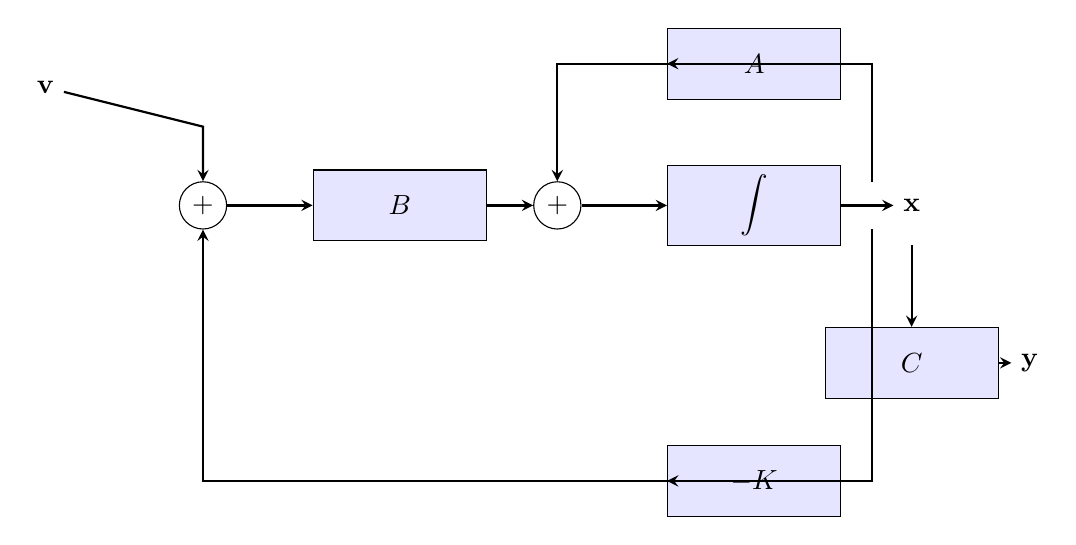
\begin{tikzpicture}[ctrlStyle/.style={draw, minimum width=2cm, minimum height=0.8cm, align=center},
    ctrlSumStyle/.style={draw, circle, inner sep=0pt, minimum size=6mm},
    ctrlBlockStyle/.style={draw, fill=blue!10, minimum width=2.2cm, minimum height=0.9cm, align=center},
    ctrlArrowStyle/.style={->, >=stealth, thick}]
    
    % Reference input node
    \node (sfV) at (0, 1.5) {$\mathbf{v}$};
    \node[ctrlSumStyle] (sum) at (2, 0) {$+$};
    \node[ctrlBlockStyle] (sfB) at (4.5, 0) {$B$};
    \node[ctrlSumStyle] (sum2) at (6.5, 0) {$+$};
    \node[ctrlBlockStyle] (int) at (9, 0) {$\displaystyle\int$};
    \node (sfX) at (11, 0) {$\mathbf{x}$};
    \node[ctrlBlockStyle] (sfC) at (11, -2) {$C$};
    \node (sfY) at (12.5, -2) {$\mathbf{y}$};
    \node[ctrlBlockStyle] (sfA) at (9, 1.8) {$A$};
    \node[ctrlBlockStyle] (sfK) at (9, -3.5) {$-K$};
    
    \draw[ctrlArrowStyle] (sfV) -- (2, 1) -- (sum.north);
    \draw[ctrlArrowStyle] (sum) -- node[above] {} (sfB);
    \draw[ctrlArrowStyle] (sfB) -- (sum2);
    \draw[ctrlArrowStyle] (sum2) -- (int);
    \draw[ctrlArrowStyle] (int) -- (sfX);
    \draw[ctrlArrowStyle] (11, -0.5) -- (sfC);
    \draw[ctrlArrowStyle] (sfC) -- (sfY);
    \draw[ctrlArrowStyle] (10.5, 0.3) |- (sfA.west);
    \draw[ctrlArrowStyle] (sfA.east) -| (sum2.north);
    \draw[ctrlArrowStyle] (10.5, -0.3) |- (sfK.west);
    \draw[ctrlArrowStyle] (sfK.east) -| (sum.south);
\end{tikzpicture}
\caption{状态反馈控制系统结构框图。状态$\mathbf{x}$通过反馈增益$-K$叠加到参考输入$\mathbf{v}$上，形成闭环动态。}
\label{fig:ch09_state_feedback_block}
\end{figure}

%%%%%%%%%%%%%%%%%%%%%%%%%%%%%%%%%%%%%%%%%%%%%%%%%%%%%%%%%%%%%%%%%%%%%%%%%%%%%%%%
\section{Ackermann公式}

\subsection{公式推导}

Ackermann公式为单输入系统提供了一种一步计算反馈增益矩阵$K$的解析方法，是极点配置问题最经典的封闭解。

\begin{myTheorem}{Ackermann公式}
对于完全能控的单输入系统$(A, B)$，若期望的闭环特征多项式为
\[
\alpha_d(s) = s^n + \alpha_{n-1}s^{n-1} + \cdots + \alpha_1 s + \alpha_0
\]
则使得闭环极点恰好为$\alpha_d(s)$的根的状态反馈增益为
\[
K = \begin{bmatrix} 0 & 0 & \cdots & 0 & 1 \end{bmatrix} \mathcal{C}^{-1} \alpha_d(A)
\]
其中$\mathcal{C} = [B, AB, \dots, A^{n-1}B]$为能控性矩阵，$\alpha_d(A)$是将多项式$\alpha_d(s)$中的$s$替换为矩阵$A$所得的矩阵多项式：
\[
\alpha_d(A) = A^n + \alpha_{n-1}A^{n-1} + \cdots + \alpha_1 A + \alpha_0 I
\]
\end{myTheorem}

\begin{proof}
利用能控标准型的性质。设变换$T$将$(A,B)$变换为能控标准型$(A_c, B_c)$，即
\[
A_c = TAT^{-1}, \quad B_c = TB
\]
其中$T = \mathcal{C}_c \mathcal{C}^{-1}$，$\mathcal{C}_c$是能控标准型的能控性矩阵。

已知在能控标准型下的反馈增益为$K_c = [\alpha_0 - a_0, \dots, \alpha_{n-1} - a_{n-1}]$。由Cayley-Hamilton定理，
\[
\alpha_d(A_c) = A_c^n + \alpha_{n-1}A_c^{n-1} + \cdots + \alpha_0 I
\]
考虑$\alpha_d(A_c)$的最后一行，它恰好等于$K_c$。因此
\[
K_c = e_n^{\top} \alpha_d(A_c)
\]
其中$e_n^{\top} = [0, \dots, 0, 1]$。在原坐标系下，
\[
K = K_c T = e_n^{\top} \alpha_d(A_c) T = e_n^{\top} T \alpha_d(A) T^{-1} T = e_n^{\top} T \alpha_d(A)
\]
而$e_n^{\top} T = e_n^{\top} \mathcal{C}_c \mathcal{C}^{-1}$。在能控标准型中，$\mathcal{C}_c$是特定的上三角矩阵，$e_n^{\top} \mathcal{C}_c = [0, \dots, 0, 1]$，从而$e_n^{\top} T = [0, \dots, 0, 1] \mathcal{C}^{-1}$，即得证。
\end{proof}

\subsection{计算步骤与应用}

利用Ackermann公式计算状态反馈增益的步骤：

\begin{myalgorithm}{Ackermann极点配置算法}
\begin{enumerate}
\item \textbf{确定期望闭环特征多项式}$\alpha_d(s) = (s - \lambda_1^{\mathrm{d}})(s - \lambda_2^{\mathrm{d}}) \cdots (s - \lambda_n^{\mathrm{d}})$，提取系数$\alpha_0, \alpha_1, \dots, \alpha_{n-1}$；
\item \textbf{构造能控性矩阵}$\mathcal{C} = [B, AB, \dots, A^{n-1}B]$，验证$\operatorname{rank}(\mathcal{C}) = n$；
\item \textbf{计算矩阵多项式}$\alpha_d(A) = A^n + \alpha_{n-1}A^{n-1} + \cdots + \alpha_1 A + \alpha_0 I$；
\item \textbf{计算反馈增益}$K = e_n^{\top} \mathcal{C}^{-1} \alpha_d(A)$。
\end{enumerate}
\end{myalgorithm}

\begin{example}[二阶系统的极点配置]
考虑系统
\[
A = \begin{bmatrix} 0 & 1 \\ 2 & 3 \end{bmatrix},\quad B = \begin{bmatrix} 0 \\ 1 \end{bmatrix}
\]
期望闭环极点为$\lambda_{1,2}^{\mathrm{d}} = -3 \pm j4$。

期望特征多项式为
\[
\alpha_d(s) = (s + 3 - j4)(s + 3 + j4) = s^2 + 6s + 25
\]
即$\alpha_1 = 6$，$\alpha_0 = 25$。

能控性矩阵：
\[
\mathcal{C} = \begin{bmatrix} 0 & 1 \\ 1 & 3 \end{bmatrix},\quad \mathcal{C}^{-1} = \begin{bmatrix} -3 & 1 \\ 1 & 0 \end{bmatrix}
\]
矩阵多项式：
\[
\alpha_d(A) = A^2 + 6A + 25I = \begin{bmatrix} 2 & 3 \\ 6 & 11 \end{bmatrix} + \begin{bmatrix} 0 & 6 \\ 12 & 18 \end{bmatrix} + \begin{bmatrix} 25 & 0 \\ 0 & 25 \end{bmatrix} = \begin{bmatrix} 27 & 9 \\ 18 & 54 \end{bmatrix}
\]
反馈增益：
\[
K = \begin{bmatrix} 0 & 1 \end{bmatrix} \begin{bmatrix} -3 & 1 \\ 1 & 0 \end{bmatrix} \begin{bmatrix} 27 & 9 \\ 18 & 54 \end{bmatrix} = \begin{bmatrix} 1 & 0 \end{bmatrix} \begin{bmatrix} 27 & 9 \\ 18 & 54 \end{bmatrix} = \begin{bmatrix} 27 & 9 \end{bmatrix}
\]
验证：$A - BK = \begin{bmatrix} 0 & 1 \\ -25 & -6 \end{bmatrix}$，其特征值为$-3 \pm j4$，与期望一致。
\end{example}

\begin{remark}
Ackermann公式在数值计算中可能不稳定（当系统阶数较高时），因为需要计算矩阵幂$A^n$，可能引入较大的舍入误差。在实际工程中，通常使用更鲁棒的数值方法（如MATLAB的\texttt{place}命令），但在低阶系统和理论分析中，Ackermann公式仍然是最清晰的解析表达。
\end{remark}

%%%%%%%%%%%%%%%%%%%%%%%%%%%%%%%%%%%%%%%%%%%%%%%%%%%%%%%%%%%%%%%%%%%%%%%%%%%%%%%%
\section{状态观测器}

当系统状态无法直接测量时，需要设计状态观测器来"估计"状态，然后用估计状态代替真实状态进行反馈控制。

\subsection{开环与闭环观测器}

\textbf{开环观测器}（Luenberger, 1964年的早期版本）直接仿真原系统：
\[
\dot{\hat{\mathbf{x}}} = A\hat{\mathbf{x}} + B\mathbf{u}
\]
其估计误差$\tilde{\mathbf{x}} = \mathbf{x} - \hat{\mathbf{x}}$满足
\[
\dot{\tilde{\mathbf{x}}} = A\tilde{\mathbf{x}}
\]
若$A$本身不稳定，则估计误差发散——这就是开环观测器的根本缺陷。

\textbf{闭环观测器（Luenberger观测器）}引入了输出估计误差的反馈修正项：
\begin{myformula}
\dot{\hat{\mathbf{x}}} = A\hat{\mathbf{x}} + B\mathbf{u} + L(\mathbf{y} - C\hat{\mathbf{x}})
\end{myformula}
其中$L \in \R^{n \times p}$是\textbf{观测器增益矩阵}。估计误差动态为
\[
\dot{\tilde{\mathbf{x}}} = (A - LC)\tilde{\mathbf{x}}
\]
只要通过设计$L$使$(A-LC)$的特征值具有充分负的实部，估计误差将渐近收敛到零。

\begin{myTheorem}{观测器极点配置（对偶原理）}
系统$(A, C)$能观的充分必要条件是：存在观测器增益$L$使得$A-LC$具有任意指定的特征值。这等价于对偶系统$(A^{\top}, C^{\top})$的能控性与极点配置问题。
\end{myTheorem}

\begin{proof}
注意到
\[
\lambda(A - LC) = \lambda((A - LC)^{\top}) = \lambda(A^{\top} - C^{\top}L^{\top})
\]
将$(A^{\top}, C^{\top})$看作状态空间的"系统"，则$L^{\top}$就扮演了"反馈增益"的角色。根据极点配置定理，存在$L^{\top}$使得$A^{\top} - C^{\top}L^{\top}$具有任意特征值的充要条件是$(A^{\top}, C^{\top})$能控，即$(A, C)$能观。因此$L$可以通过对偶系统的Ackermann公式或\texttt{place}命令计算。
\end{proof}

\subsection{观测器增益的设计}

对偶系统的Ackermann公式：对于单输出系统（$p=1$），若期望观测器特征多项式为$\beta_d(s) = s^n + \beta_{n-1}s^{n-1} + \cdots + \beta_0$，则
\[
L^{\top} = \begin{bmatrix} 0 & 0 & \cdots & 1 \end{bmatrix} \mathcal{O}^{-1} \beta_d(A^{\top})
\]
其中$\mathcal{O}$为能观性矩阵$[C^{\top}, A^{\top}C^{\top}, \dots, (A^{\top})^{n-1}C^{\top}]^{\top}$。

观测器极点的选择原则：
\begin{enumerate}
\item 观测器极点应比控制器极点具有更负的实部（通常快3--5倍），以保证估计误差的衰减远快于系统动态；
\item 但若观测器极点过于远离虚轴，观测器增益会很大，导致噪声放大严重，形成"噪声峰值"效应；
\item 工程实践中需在估计速度与噪声敏感性之间进行折中。
\end{enumerate}

\begin{figure}[H]
\centering
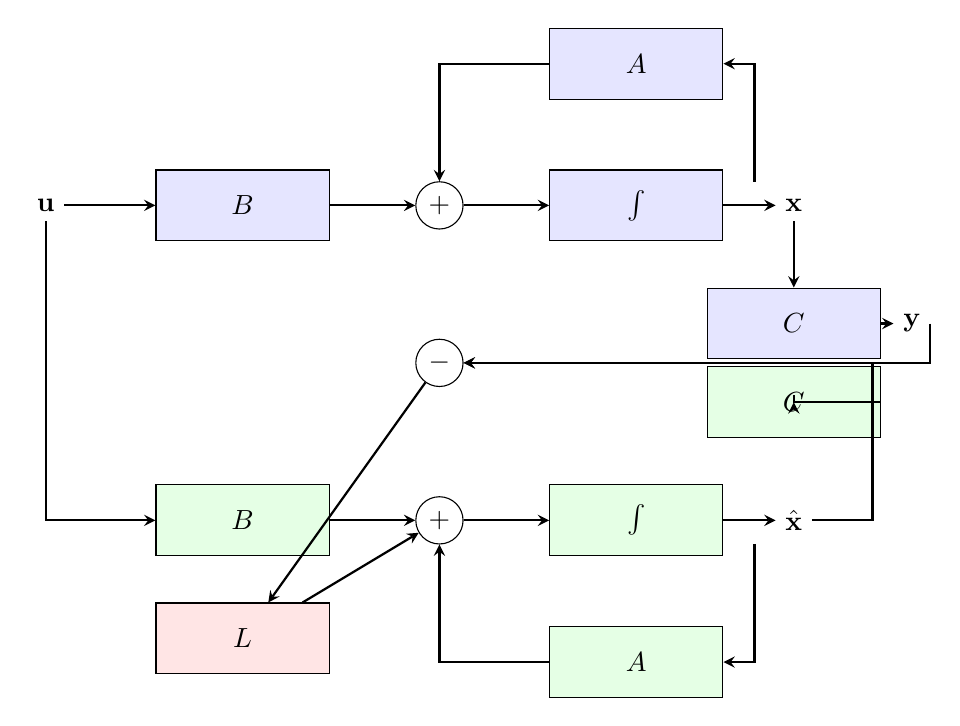
\begin{tikzpicture}[ctrlObsStyle/.style={draw, minimum width=2cm, minimum height=0.8cm, align=center},
    ctrlObsSum/.style={draw, circle, inner sep=0pt, minimum size=6mm},
    ctrlObsBlock/.style={draw, fill=green!10, minimum width=2.2cm, minimum height=0.9cm, align=center},
    ctrlObsArrow/.style={->, >=stealth, thick}]
    
    % Plant
    \node[ctrlObsBlock, fill=blue!10] (plantB) at (3, 2) {$B$};
    \node[ctrlObsSum] (plantSum) at (5.5, 2) {$+$};
    \node[ctrlObsBlock, fill=blue!10] (plantInt) at (8, 2) {$\int$};
    \node (plantX) at (10, 2) {$\mathbf{x}$};
    \node[ctrlObsBlock, fill=blue!10] (plantA) at (8, 3.8) {$A$};
    \node[ctrlObsBlock, fill=blue!10] (plantC) at (10, 0.5) {$C$};
    \node (plantY) at (11.5, 0.5) {$\mathbf{y}$};
    
    % Observer
    \node[ctrlObsBlock, fill=green!10] (obsB) at (3, -2) {$B$};
    \node[ctrlObsSum] (obsSum) at (5.5, -2) {$+$};
    \node[ctrlObsBlock, fill=green!10] (obsInt) at (8, -2) {$\int$};
    \node (obsXhat) at (10, -2) {$\hat{\mathbf{x}}$};
    \node[ctrlObsBlock, fill=green!10] (obsA) at (8, -3.8) {$A$};
    \node[ctrlObsBlock, fill=green!10] (obsC) at (10, -0.5) {$C$};
    \node[ctrlObsSum] (obsErr) at (5.5, 0) {$-$};
    \node[ctrlObsBlock, fill=red!10] (obsL) at (3, -3.5) {$L$};
    
    \node (u) at (0.5, 2) {$\mathbf{u}$};
    
    \draw[ctrlObsArrow] (u) -- (plantB);
    \draw[ctrlObsArrow] (plantB) -- (plantSum);
    \draw[ctrlObsArrow] (plantSum) -- (plantInt);
    \draw[ctrlObsArrow] (plantInt) -- (plantX);
    \draw[ctrlObsArrow] (plantX) -- (plantC);
    \draw[ctrlObsArrow] (plantC) -- (plantY);
    \draw[ctrlObsArrow] (9.5, 2.3) |- (plantA.east);
    \draw[ctrlObsArrow] (plantA.west) -| (plantSum.north);
    
    \draw[ctrlObsArrow] (u) |- (obsB);
    \draw[ctrlObsArrow] (obsB) -- (obsSum);
    \draw[ctrlObsArrow] (obsSum) -- (obsInt);
    \draw[ctrlObsArrow] (obsInt) -- (obsXhat);
    \draw[ctrlObsArrow] (9.5, -2.3) |- (obsA.east);
    \draw[ctrlObsArrow] (obsA.west) -| (obsSum.south);
    
    \draw[ctrlObsArrow] (plantY.east) |- (11.7, 0) |- (obsErr.east);
    \draw[ctrlObsArrow] (obsXhat) -- (11.0, -2) |- (10, -0.5) -- (obsC);
    \draw[ctrlObsArrow] (obsC) -- (11.0, -0.5) |- (obsErr.east);
    \draw[ctrlObsArrow] (obsErr) -- (obsL);
    \draw[ctrlObsArrow] (obsL) -- (obsSum);
\end{tikzpicture}
\caption{Luenberger状态观测器结构。观测器复制了被控对象的结构，并通过估计误差$\mathbf{y} - C\hat{\mathbf{x}}$经增益$L$进行反馈修正。}
\label{fig:ch09_luenberger_observer}
\end{figure}

%%%%%%%%%%%%%%%%%%%%%%%%%%%%%%%%%%%%%%%%%%%%%%%%%%%%%%%%%%%%%%%%%%%%%%%%%%%%%%%%
\section{分离原理}

\subsection{控制器与观测器的独立设计}

分离原理（Separation Principle）是现代控制理论中最优美的结果之一，它表明：状态反馈控制器和状态观测器可以\textbf{独立设计}，组合后整个闭环系统的极点集合恰好是控制器极点与观测器极点的并集。

考虑基于观测器的状态反馈：
\[
\mathbf{u} = -K\hat{\mathbf{x}} + \mathbf{v}
\]
其中$\hat{\mathbf{x}}$由Luenberger观测器提供。闭环增广系统的状态为$[\mathbf{x}^{\top}, \tilde{\mathbf{x}}^{\top}]^{\top}$，其中$\tilde{\mathbf{x}} = \mathbf{x} - \hat{\mathbf{x}}$。状态空间方程为：

\begin{myformula}
\frac{d}{dt}\begin{bmatrix} \mathbf{x} \\ \tilde{\mathbf{x}} \end{bmatrix} =
\begin{bmatrix}
A - BK & BK \\
0 & A - LC
\end{bmatrix}
\begin{bmatrix} \mathbf{x} \\ \tilde{\mathbf{x}} \end{bmatrix} +
\begin{bmatrix} B \\ 0 \end{bmatrix} \mathbf{v}
\end{myformula}

\begin{myTheorem}{分离原理}
增广系统的特征值为
\[
\lambda\left(\begin{bmatrix} A-BK & BK \\ 0 & A-LC \end{bmatrix}\right) = \lambda(A-BK) \cup \lambda(A-LC)
\]
即闭环系统的极点恰好是状态反馈极点（由$K$决定）与观测器极点（由$L$决定）的并集。
\end{myTheorem}

\begin{proof}
由于增广系统矩阵是上三角块矩阵，其特征多项式为
\[
\det\begin{bmatrix} sI - (A-BK) & -BK \\ 0 & sI - (A-LC) \end{bmatrix} = \det(sI - (A-BK)) \cdot \det(sI - (A-LC))
\]
\end{proof}

\begin{remark}
分离原理的工程意义极为深远：控制器增益$K$的设计可以假定全部状态可测（按理想情况配置极点），观测器增益$L$的设计可以独立进行（按误差衰减速度要求配置），两者互不干扰。这极大地简化了实际控制系统的设计流程。
\end{remark}

\begin{figure}[H]
\centering
\begin{tikzpicture}[sepStyle/.style={draw, minimum width=2.5cm, minimum height=0.9cm, align=center},
    sepSum/.style={draw, circle, inner sep=0pt, minimum size=6mm},
    sepBlock/.style={draw, fill=blue!10, minimum width=2.5cm, minimum height=0.9cm, align=center},
    sepObs/.style={draw, fill=green!10, minimum width=2.5cm, minimum height=0.9cm, align=center},
    sepArrow/.style={->, >=stealth, thick},
    sepDashArrow/.style={->, >=stealth, thick, dashed}]
    
    \node[sepBlock] (controller) at (0, 0) {状态反馈\\$-K$};
    \node[sepBlock, fill=red!10] (plant) at (5, 0) {被控对象\\$A, B, C$};
    \node[sepObs] (observer) at (5, -3.5) {Luenberger\\观测器};
    
    \draw[sepArrow] (-3.5, 0) -- node[above] {$\mathbf{v}$} (controller);
    \draw[sepArrow] (controller) -- node[above] {$\mathbf{u}$} (plant);
    \draw[sepArrow] (plant.east) -- ++(1, 0) node[right] {$\mathbf{y}$};
    \draw[sepDashArrow] (observer.west) -| node[below, pos=0.3] {$\hat{\mathbf{x}}$} (controller.south);
    \draw[sepArrow] (plant.south) |- (observer.east);
    \draw[sepArrow] (controller.south) |- (3, -1.5) |- node[above, pos=0.2] {$\mathbf{u}$} (observer.north);
    
    \node[sepStyle, draw=none] at (5, -5) {\textbf{分离原理：}$K$和$L$可独立设计};
\end{tikzpicture}
\caption{分离原理示意图。控制器增益$K$和观测器增益$L$可以独立设计：$K$假设全状态可测，按理想极点配置；$L$按误差衰减速度设计。}
\label{fig:ch09_separation_principle}
\end{figure}

\subsection{观测器增益的极点配置（对偶设计）}

观测器增益$L$的设计可通过对偶系统的Ackermann公式或直接利用极点配置算法完成。对于单输出系统，设期望的观测器特征多项式为
\[
\beta_d(s) = (s - \mu_1)(s - \mu_2) \cdots (s - \mu_n) = s^n + \beta_{n-1}s^{n-1} + \cdots + \beta_0
\]
其中$\mu_i$是期望的观测器极点（应远大于主导控制器极点的实部）。

利用对偶性，将原系统$(A, C)$的对偶系统$(A^{\top}, C^{\top})$视为"需配置极点的系统"，利用Ackermann公式计算：
\[
L^{\top} = e_n^{\top} \mathcal{O}_d^{-1} \beta_d(A^{\top})
\]
其中$\mathcal{O}_d = [C^{\top}, A^{\top}C^{\top}, \dots, (A^{\top})^{n-1}C^{\top}]$。

\begin{example}[倒立摆的状态观测器]
考虑倒立摆的线性化模型：
\[
A = \begin{bmatrix} 0 & 1 \\ \frac{g}{\ell} & 0 \end{bmatrix},\quad
C = \begin{bmatrix} 1 & 0 \end{bmatrix}
\]
其中$g = 9.81$，$\ell = 0.5$。设计观测器使估计误差衰减的极点位于$\mu_{1,2} = -6 \pm j0$。

期望特征多项式为$\beta_d(s) = (s+6)^2 = s^2 + 12s + 36$。利用对偶Ackermann公式可得观测器增益$L$。
\end{example}

%%%%%%%%%%%%%%%%%%%%%%%%%%%%%%%%%%%%%%%%%%%%%%%%%%%%%%%%%%%%%%%%%%%%%%%%%%%%%%%%
\section{基于观测器的输出反馈}

\subsection{完整结构}

基于观测器的输出反馈控制系统由三部分组成：被控对象、状态观测器和状态反馈控制器。其数学描述为：

\textbf{被控对象}：
\[
\dot{\mathbf{x}} = A\mathbf{x} + B\mathbf{u},\quad \mathbf{y} = C\mathbf{x}
\]

\textbf{Luenberger观测器}：
\[
\dot{\hat{\mathbf{x}}} = A\hat{\mathbf{x}} + B\mathbf{u} + L(\mathbf{y} - C\hat{\mathbf{x}})
\]

\textbf{控制律}：
\[
\mathbf{u} = -K\hat{\mathbf{x}} + \mathbf{v}
\]

综合以上方程，可得从参考输入$\mathbf{v}$到输出$\mathbf{y}$的闭环传递函数。值得注意的重要事实是：

\begin{myTheorem}{传递函数的等价性}
基于观测器的输出反馈控制系统的传递函数（从$\mathbf{v}$到$\mathbf{y}$）等于直接状态反馈控制系统的传递函数。即观测器的引入\textbf{不改变}输入-输出关系。
\end{myTheorem}

\begin{proof}
计算闭环传递函数。观测器方程可写为
\[
\dot{\hat{\mathbf{x}}} = (A - BK - LC)\hat{\mathbf{x}} + L\mathbf{y} + B\mathbf{v}
\]
经过拉普拉斯变换并消去$\hat{\mathbf{x}}$，可以证明$\mathbf{Y}(s) = C(sI - A + BK)^{-1}B\,\mathbf{V}(s)$，与直接状态反馈一致。
\end{proof}

这一性质有两层含义：理论上它体现了分离原理的优雅；实践上它意味着观测器动态不影响从参考输入到输出的稳态增益和传递零点。

\subsection{传递函数的实现——二自由度结构}

基于观测器的输出反馈可以重新组织为一种"二自由度"结构。定义控制器传递函数$K(s)$：
\[
K(s) = K(sI - A + BK + LC)^{-1}L
\]
则控制信号为
\[
\mathbf{U}(s) = K(s)\mathbf{Y}(s) + \mathbf{V}(s)
\]
这意味着整个控制系统等价于一个动态输出反馈控制器。$K(s)$被称为\textbf{基于观测器的控制器}。

\begin{figure}[H]
\centering
\begin{tikzpicture}[obsCtrlStyle/.style={draw, minimum width=2.5cm, minimum height=0.9cm, align=center},
    obsCtrlSum/.style={draw, circle, inner sep=0pt, minimum size=6mm},
    obsCtrlBlock/.style={draw, fill=orange!15, minimum width=2.5cm, minimum height=0.9cm, align=center},
    obsCtrlArrow/.style={->, >=stealth, thick}]
    
    \node[obsCtrlBlock] (ctrl) at (0, 0) {观测器\\$K(s)$};
    \node[obsCtrlBlock, fill=blue!10] (plant) at (5.5, 0) {$G(s)$\\被控对象};
    \node[obsCtrlSum] (sum) at (-3, 0) {$+$};
    \node[obsCtrlSum] (sum2) at (-3, 2.5) {$-$};
    
    \draw[obsCtrlArrow] (-5.5, 0) -- node[above] {$\mathbf{v}$} (sum);
    \draw[obsCtrlArrow] (sum) -- (ctrl);
    \draw[obsCtrlArrow] (ctrl) -- node[above] {$\mathbf{u}$} (plant);
    \draw[obsCtrlArrow] (plant.east) -- ++(1.5, 0) node[right] {$\mathbf{y}$};
    \draw[obsCtrlArrow] (7, -0.3) |- (7, -1.5) -- (3, -1.5) |- (ctrl.south);
    
    \draw (-5.5, 2.5) node {$\mathbf{r}$};
    \draw[obsCtrlArrow] (-5.5, 2.5) -- (sum2);
    \draw[obsCtrlArrow] (sum2) -- (sum);
\end{tikzpicture}
\caption{基于观测器的输出反馈控制系统的等效二自由度结构。$K(s)$是基于观测器的动态控制器，实现了参考输入$\mathbf{r}$（前馈）和输出$\mathbf{y}$（反馈）的双通道处理。}
\label{fig:ch09_observer_output_feedback}
\end{figure}

%%%%%%%%%%%%%%%%%%%%%%%%%%%%%%%%%%%%%%%%%%%%%%%%%%%%%%%%%%%%%%%%%%%%%%%%%%%%%%%%
\section{MATLAB与Python实现}

\subsection{MATLAB实现}

MATLAB提供了\texttt{place}和\texttt{acker}两个命令用于极点配置。\texttt{place}基于特征结构配置的数值算法，适用于多输入系统和病态系统；\texttt{acker}是Ackermann公式的实现，仅适用于单输入系统。

\begin{mycode}{MATLAB极点配置示例}
\begin{lstlisting}[language=Matlab]
% 系统定义
A = [0 1 0; 0 0 1; -2 -3 -5];
B = [0; 0; 1];
C = [1 0 0];
D = 0;

% 期望极点
p_des = [-3+4j, -3-4j, -10];

% 验证能控性
Co = ctrb(A, B);
rank_Co = rank(Co);  % 应为3

% 状态反馈增益（多输入系统推荐place）
K = place(A, B, p_des);

% 验证闭环极点
eig(A - B*K)

% 观测器设计（对偶方法）
p_obs = [-15, -15, -15];  % 观测器极点（快5倍）
L = place(A', C', p_obs)';
eig(A - L*C)
\end{lstlisting}
\end{mycode}

\subsection{Python实现}

在Python中，可利用\texttt{scipy.signal}的\texttt{place\_poles}或\texttt{control}库实现极点配置。

\begin{mycode}{Python极点配置与观测器设计}
\begin{lstlisting}[language=Python]
import numpy as np
from scipy import linalg, signal

# 系统矩阵
A = np.array([[0, 1, 0],
              [0, 0, 1],
              [-2, -3, -5]])
B = np.array([[0], [0], [1]])
C = np.array([[1, 0, 0]])

# 期望极点
p_des = np.array([-3+4j, -3-4j, -10])

# 方法一：scipy.signal.place_poles
result = signal.place_poles(A, B, p_des)
K_scipy = result.gain_matrix
print(f"K (scipy) = {K_scipy}")

# 方法二：Ackermann公式（手动实现）
def ackermann(A, B, p_des):
    n = A.shape[0]
    poly = np.poly(p_des)  # 期望特征多项式的系数
    alpha_dA = np.zeros_like(A)
    for i, coeff in enumerate(poly):
        alpha_dA += coeff * np.linalg.matrix_power(A, n - i)
    C_ctrb = np.hstack([np.linalg.matrix_power(A, i) @ B
                        for i in range(n)])
    K = (np.linalg.inv(C_ctrb)[-1, :]) @ alpha_dA
    return K.reshape(1, -1)

K_acker = ackermann(A, B, p_des)
print(f"\nK (Ackermann) = {K_acker}")

# 观测器设计
p_obs = np.array([-15, -15, -15])
L = signal.place_poles(A.T, C.T, p_obs).gain_matrix.T
print(f"\nL = \n{L}")

# 验证闭环极点
print(f"\n控制器极点: {np.linalg.eigvals(A - B @ K_scipy)}")
print(f"观测器极点: {np.linalg.eigvals(A - L @ C)}")
\end{lstlisting}
\end{mycode}

\begin{mycode}{Python基于观测器的闭环仿真}
\begin{lstlisting}[language=Python]
import numpy as np
from scipy.integrate import solve_ivp
import matplotlib.pyplot as plt

# 系统参数
A = np.array([[0, 1], [9.81/0.5, 0]])  # 倒立摆
B = np.array([[0], [1/0.5]])
C = np.array([[1, 0]])

# 控制器设计
p_ctrl = np.array([-3+4j, -3-4j])
K, _, _ = signal.place_poles(A, B, p_ctrl).gain_matrix, None, None

# 观测器设计
p_obs = np.array([-15, -15])
L = signal.place_poles(A.T, C.T, p_obs).gain_matrix.T

# 增广系统
n = A.shape[0]
A_aug = np.block([
    [A, -B @ K],
    [L @ C, A - B @ K - L @ C]
])
B_aug = np.block([[B], [B]])

# 仿真
def sys_dyn(t, z):
    return A_aug @ z + B_aug.flatten() * np.sin(t)  # 正弦参考

t_span = (0, 10)
z0 = np.array([0.1, 0, 0, 0])
sol = solve_ivp(sys_dyn, t_span, z0, max_step=0.01)

x = sol.y[:2]
xhat = sol.y[2:]

fig, axes = plt.subplots(2, 1)
axes[0].plot(sol.t, x[0], 'b', label=r'$x_1$ (true)')
axes[0].plot(sol.t, xhat[0], 'r--', label=r'$\hat{x}_1$ (est)')
axes[0].legend()
axes[0].set_ylabel('Position')
axes[1].plot(sol.t, x[1], 'b', label=r'$x_2$ (true)')
axes[1].plot(sol.t, xhat[1], 'r--', label=r'$\hat{x}_2$ (est)')
axes[1].legend()
axes[1].set_ylabel('Velocity')
axes[1].set_xlabel('Time [s]')
plt.show()
\end{lstlisting}
\end{mycode}

\begin{remark}
Python的\texttt{control}库也提供了\texttt{place}和\texttt{acker}的直接调用接口，需要安装\texttt{python-control}包。上述代码使用了\texttt{scipy.signal.place\_poles}作为替代方案，该方法基于Kautsky-Nichols-Van Dooren算法，具有更好的数值稳定性。
\end{remark}

%%%%%%%%%%%%%%%%%%%%%%%%%%%%%%%%%%%%%%%%%%%%%%%%%%%%%%%%%%%%%%%%%%%%%%%%%%%%%%%%
\section{小结}

本章从状态反馈的基本概念出发，系统阐述了极点配置的理论基础与实现方法。核心结论包括：
\begin{enumerate}
\item \textbf{极点配置定理}：能控性是任意配置闭环极点的充要条件，为状态反馈设计提供了理论保障；
\item \textbf{Ackermann公式}：给出了单输入系统反馈增益的解析表达，具有重要的理论意义；
\item \textbf{对偶原理}：将观测器设计问题转化为对偶系统的极点配置问题，统一了控制器和观测器的方法论；
\item \textbf{分离原理}：控制器和观测器可独立设计，组合后整个系统的极点集为两者的并集，大大简化了工程实现。
\end{enumerate}

极点配置方法为线性系统控制设计提供了完整的理论框架。但在实际应用中，如何兼顾性能指标（如控制能量、鲁棒性等）仍是重要课题。下一章将介绍线性二次型最优控制，它在极点配置的基础上进一步引入了性能优化的思想。
